\section{Virtual Research Environments for Mathematics: the Math-in-the-Middle
  Approach}\label{sec:mmtmitm}

The work reported in this paper originates from in the EU-funded OpenDreamKit
\cite{OpenDreamKit:on} project that aims to create Virtual Research Environments (VRE)
enabling mathematicians to make efficient use of existing Open-Source mathematical
knowledge systems.  These systems include computer algebra systems like SageMath and GAP
as well as mathematical data bases such as the \lmfdb, which must be made interoperable
for integration into a VRE. In the OpenDreamKit project we have developed the
Math-in-the-Middle (MitM) approach, which posits a central ontology of mathematical
knowledge, which acts as a pivot point for interoperability; see~\cite{DehKohKon:iop16}
for a description of the approach and \cite{KohMuePfe:kbimss17} for a technical refinement
and large-scale interoperability case study. 

\begin{wrapfigure}l{0.3\textwidth}%\vspace*{-2em}
    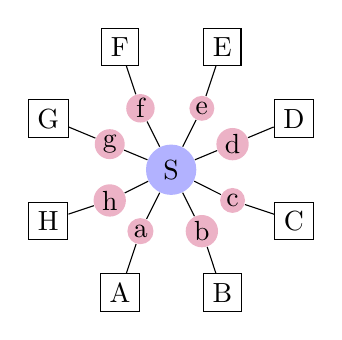
\begin{tikzpicture}[xscale=1.3,yscale=1.3]\normalsize
      \tikzstyle{withshadow}=[draw,drop shadow={opacity=.5},fill=white]
      \tikzstyle{system}=[draw]
      \tikzstyle{standard}=[circle,fill=blue!30]
      \tikzstyle{interface}=[circle,fill=purple!30,inner sep = 1pt,]
      \node[system] (a) at (0,.3) {A};
      \node[system] (b) at (1,.3) {B};
      \node[system] (c) at (1.7,1) {C};
      \node[system] (d) at (1.7,2) {D};
      \node[system] (e) at (1,2.7) {E};
      \node[system] (f) at (0,2.7) {F};
      \node[system] (g) at (-.7,2) {G};
      \node[system] (h) at (-.7,1) {H};
      \node[standard] (m) at (.5,1.5) {S};
      \node[interface] (ia) at (0.2,.9) {a};
      \node[interface] (ib) at (.8,.9) {b};
      \node[interface] (ic) at (1.1,1.2) {c};
      \node[interface] (id) at (1.1,1.75) {d};
      \node[interface] (ie) at (.8,2.1) {e};
      \node[interface] (if) at (0.2,2.1) {f};
      \node[interface] (ig) at (-.1,1.75) {g};
      \node[interface] (ih) at (-.1,1.2) {h};
      \draw (m) -- (ia) -- (a);
      \draw (m) -- (ib) -- (b);
      \draw (m) -- (ic) -- (c);
      \draw (m) -- (id) -- (d);
      \draw (m) -- (ie) -- (e);
      \draw (m) -- (if) -- (f);
      \draw (m) -- (ig) -- (g);
      \draw (m) -- (ih) -- (h);
      \end{tikzpicture}
  \caption{The MiTM Approach to Connecting Systems.}\label{fig:mitmconnect}\vspace*{-1em}
\end{wrapfigure}
The MitM ontology in the center of Figure~\ref{fig:mitmconnect} models the true,
underlying mathematical semantics in \ommt and allows translation between this centrally
formalized knowledge and the systems on the boundary via views and alignments.
This mathematical knowledge is modeled using the well-established theory graph paradigm
and is stored inside our \ommt-based MathHub system~\cite{MathHub:on}. 

The knowledge in the mathematical software systems -- denoted by square boxes in
Figure~\ref{fig:mitmconnect} -- also modeled via \ommt theory graphs the \textbf{API
  Content Dictionaries} -- the corresponding red circles; these are generated from the
knowledge bases in the systems by a custom process. The API CDs allow us to implement
translation with the help of \ommt views and alignments between the ontology -- the
Math-In-The-Middle -- and each of the systems and use these translations for transporting
computational tasks between the systems. 

The realization of the MitM approach crucially depends on the information architecture of
the \ommt language~\cite{Kohlhase:OMDoc1.2,RabKoh:WSMSML13} and its implementation in the
\mmt system~\cite{Rabe:MAGMS13,uniformal:on}.

In \ommt knowledge is organized in \textbf{theories}, which contain information about
mathematical concepts and objects in the form of \textbf{declarations}. Theories are
organized into an ``object-oriented'' inheritance structure via \textbf{inclusions} and
\textbf{structures} (for controlled multiple inheritance), which is augmented via
truth-preserving mappings between theories called \textbf{views}, which allow to relate
concepts of pre-existing theories and transport theorems between these. Inclusions,
structures, and views impose a graph structure on the represented mathematical knowledge,
called a \textbf{theory graph}. 

We observe that even very large mathematical knowledge spaces about abstract mathematical
domains can be represented by small, but densely connected, theory graphs, if we make all
inherited material explicit in a process called \textbf{flattening}. The \ommt language
provides systematic names (\mmt URIs) for all objects, properties, and relations in the
induced knowledge space, and given the represented theory graph, the \mmt system can
compute them by need. 

Generally, knowledge in a knowledge space given by a theory graph loaded by the \mmt
system can be accessed by either giving it's \mmt URI, or by giving a set of conditions
that has to fulfilled by the knowledge in question. The achieve the latter, \mmt has a
Query Language called QMT~\cite{Rabe:qlfml12}, which allows even complex conditions to be
specified. Concretely, the \mmt system loads the theory graph into main memory at startup
and interleaves incremental flattening and query evaluation operations on the \mmt data
structures until the result has been produced. 

In \cite{KohMuePfe:kbimss17} we show that the MitM approach, its \ommt-based realization,
and distribution via the SCSCP protocol are sufficient distributed, federated computation
between multiple computer algebra systems (Sage, GAP, and Singular), and that the MitM
ontology of abstract group theory can be represented in \ommt efficiently. This setup is
effective because
\begin{compactenum}[\bf C1]
\item the knowledge spaces behind abstract and computational mathematics can be
  represented in theory graphs very space-efficiently: The compression factors between a
  knowledge space and its theory graph -- we call it the \textbf{TG factor}\ednote{MK@FR:
    we should have a name for that factor; something like the ``deBruijn factor''; only
    that we want it to be large! I think we should talk about this on the tetrapod meeting
    and jointly decide on one and argue with that; I will use TG factor for now.} --
  exceed two orders of magnitude even for small domains.
\item only small parts of the knowledge space are traversed for a given computation. 
\end{compactenum}

But the OpenDreamKit VRE must also include mathematical data sources like the \lmfdb or
the OEIS, which contain millions of mathematical objects. For such knowledge sources, the
classical \mmt system is not yet suitable: 
\begin{compactenum}[\bf V1]
\item the knowledge space corresponding to the data base content cannot be compressed by
  ``general mathematical principles'' like inheritance. Indeed, redundant information is
  already largely eliminated by the data base schema and the ``business logic'' of the
  information system.
\item typically large parts of the knowledge space need to be traversed to obtain the
  intended results to queries.
\end{compactenum}
As a consequence, we extend the concept of \ommt theories -- which carry the implicit
assumption of containing only a small number of declarations (see~\cite{FaGu:lt92} for a
discussion) -- to \textbf{virtual theories}, which can have an unlimited number of
declarations or -- while we are at it -- even infinitely many. To contrast the intended
uses we will call the classical \ommt theories \textbf{concrete theories}. 

From a system perspective, virtual theories behave just like concrete theories, but
without the assumption of loading all declarations from a file on disk at system startup.
Instead of loading all knowledge from an XML file, virtual theories load declarations in a
lazy fashion when they are required.  Here we do not even restrict ourselves to lazily
reading an XML file, on the contrary, in most use cases we actually create the \ommt
representation on demand.

%%% Local Variables:
%%% mode: latex
%%% TeX-master: "paper"
%%% End:

%  LocalWords:  omdocmmt fig:classicalconnect fig:mitmconnect OpenDreamKit:on lmfdb lmfdb
%  LocalWords:  ODKproposal:on DehKohKon:iop16 sagemath oeis fig:mitmontology colored ig
%  LocalWords:  mathrm mathrm sec:mmtmitm ommt mechanized uniformal:on organized textit
%  LocalWords:  BusCapCar:oms04 MathHub:on Iancu:phd SMGloM:on formalizations wrapfigure
%  LocalWords:  PVSlibraries:on mizar:online textwidth tikzpicture xscale 1.3,yscale
%  LocalWords:  tikzstyle withshadow draw,drop circle,fill 30,inner formalized vspace
%  LocalWords:  MACIS17-interop KohMuePfe:kbimss17 1.3,yscale 30,inner fit:mitmconnect
%  LocalWords:  textbf realization RabKoh:WSMSML13 Rabe:MAGMS13,uniformal:on Rabe:qlfml12
%  LocalWords:  FaGu:lt92
